\section{ueac Struct Reference}
\label{structueac}\index{ueac@{ueac}}
{\tt \#include $<$ueac.h$>$}

Collaboration diagram for ueac:\begin{figure}[H]
\begin{center}
\leavevmode
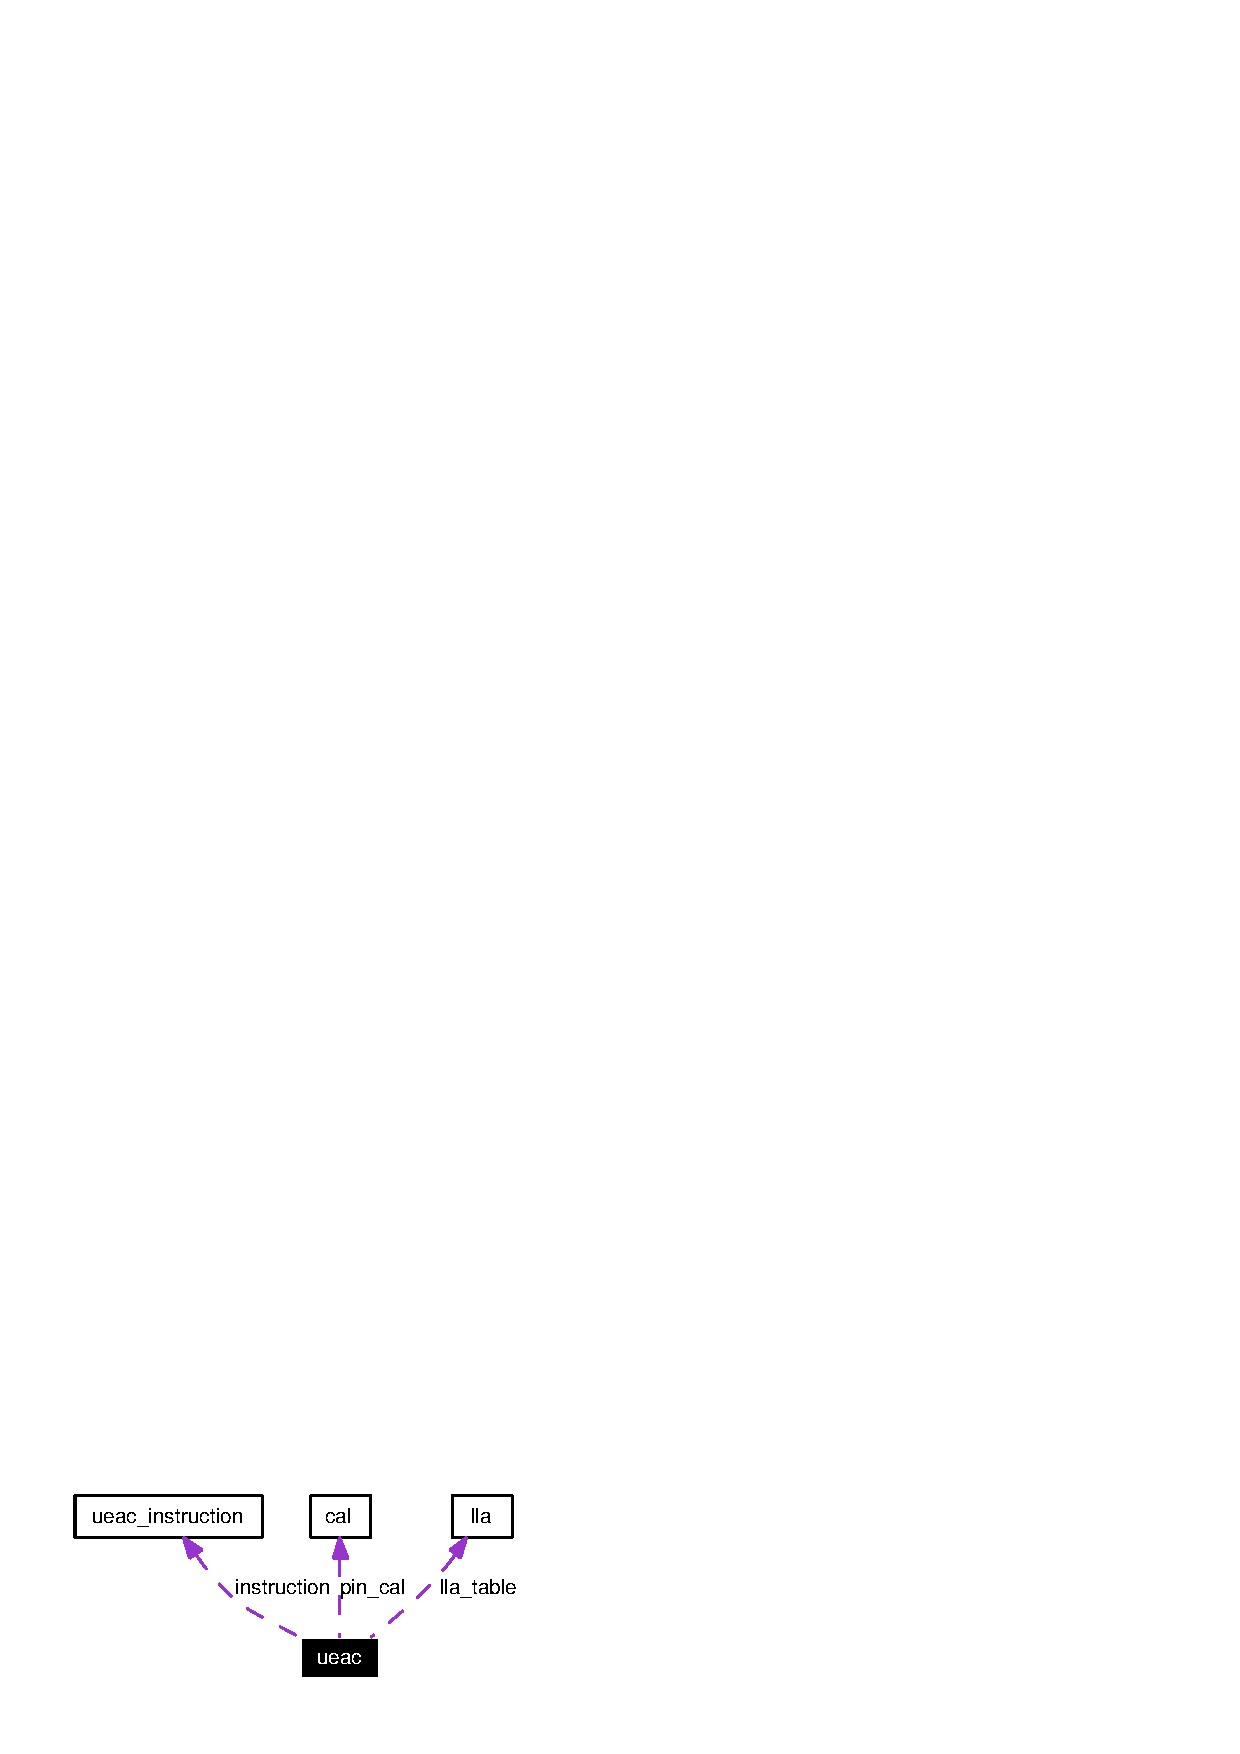
\includegraphics[width=135pt]{structueac__coll__graph}
\end{center}
\end{figure}
\subsection*{Data Fields}
\begin{CompactItemize}
\item 
{\bf ueac\_\-instruction\_\-t} {\bf instruction}
\item 
unsigned long {\bf lla\_\-input}
\item 
unsigned short {\bf pin\_\-current} [25]
\item 
{\bf cal\_\-t} {\bf pin\_\-cal} [25]
\item 
{\bf lla\_\-t} {\bf lla\_\-table} [10]
\end{CompactItemize}


\subsection{Detailed Description}




Definition at line 107 of file ueac.h.

\subsection{Field Documentation}
\index{ueac@{ueac}!instruction@{instruction}}
\index{instruction@{instruction}!ueac@{ueac}}
\subsubsection{\setlength{\rightskip}{0pt plus 5cm}{\bf ueac\_\-instruction\_\-t} {\bf ueac::instruction}}\label{structueac_o0}




Definition at line 108 of file ueac.h.

Referenced by interpreter(), report\_\-instruction(), and ueac\_\-execute\_\-instruction().\index{ueac@{ueac}!lla_input@{lla\_\-input}}
\index{lla_input@{lla\_\-input}!ueac@{ueac}}
\subsubsection{\setlength{\rightskip}{0pt plus 5cm}unsigned long {\bf ueac::lla\_\-input}}\label{structueac_o1}




Definition at line 109 of file ueac.h.

Referenced by init\_\-ueac\_\-state\_\-structure(), lla\_\-add(), lla\_\-disable(), lla\_\-enable(), lla\_\-input\_\-check(), and lla\_\-print\_\-active().\index{ueac@{ueac}!lla_table@{lla\_\-table}}
\index{lla_table@{lla\_\-table}!ueac@{ueac}}
\subsubsection{\setlength{\rightskip}{0pt plus 5cm}{\bf lla\_\-t} {\bf ueac::lla\_\-table}[10]}\label{structueac_o4}




Definition at line 112 of file ueac.h.

Referenced by init\_\-ueac\_\-state\_\-structure().\index{ueac@{ueac}!pin_cal@{pin\_\-cal}}
\index{pin_cal@{pin\_\-cal}!ueac@{ueac}}
\subsubsection{\setlength{\rightskip}{0pt plus 5cm}{\bf cal\_\-t} {\bf ueac::pin\_\-cal}[25]}\label{structueac_o3}




Definition at line 111 of file ueac.h.

Referenced by convert\_\-a2d(), current\_\-output\_\-calibration(), init\_\-ueac\_\-state\_\-structure(), and write\_\-current().\index{ueac@{ueac}!pin_current@{pin\_\-current}}
\index{pin_current@{pin\_\-current}!ueac@{ueac}}
\subsubsection{\setlength{\rightskip}{0pt plus 5cm}unsigned short {\bf ueac::pin\_\-current}[25]}\label{structueac_o2}




Definition at line 110 of file ueac.h.

Referenced by init\_\-ueac\_\-state\_\-structure(), and ueac\_\-execute\_\-instruction().

The documentation for this struct was generated from the following file:\begin{CompactItemize}
\item 
{\bf ueac.h}\end{CompactItemize}
